\setcounter{section}{3}
\setcounter{subsection}{3}
\setcounter{subsubsection}{1}
\subsubsection{The rate monotonic schedule.}

\begin{enumerate}[label=\textbf{\arabic*})]
\item \textbf{Calculating utilization}

The utilization of a periodic task $\tau_i(T_i,C_i)$ is defined as:
\[u_i = \frac{C_i}{T_i}\]
The total utilization for a set of tasks is defined as:
\[U = \sum_{i=1}^{n} u_i\]

The 3 tasks given are:
\[\tau_i(\phi_i, T_i, C_i, D_i)\]

\[\tau_1(100, 300, 100, 300)\]
\[\tau_2(100, 400, 100, 400)\]
\[\tau_3(100, 600, 100, 600)\]

Their respective utilizations are:
\[u_1 = \frac{C_1}{D_1} = \frac{100}{300} = \frac{1}{3}\]
\[u_2 = \frac{C_2}{D_2} = \frac{100}{400} = \frac{1}{4}\]
\[u_3 = \frac{C_3}{D_3} = \frac{100}{600} = \frac{1}{6}\]

The total utilization $U$ can thus be calculated:
\[U = \frac{1}{3} + \frac{1}{4} + \frac{1}{6} = \frac{9}{12} = \frac{3}{4} = 0.75\]

The hyperperiod $H$ is defined as the least common multiplier from the set of task periods:
\[H = lcm(T_1, T_2, T_3) = lcm (300, 400, 600) = 1200\]

According to RMS the priorities should therefore be:
\[P_1 > P_2 > P_3\]

For one hyperperiod of 1200ms the ideal schedule looks like this:

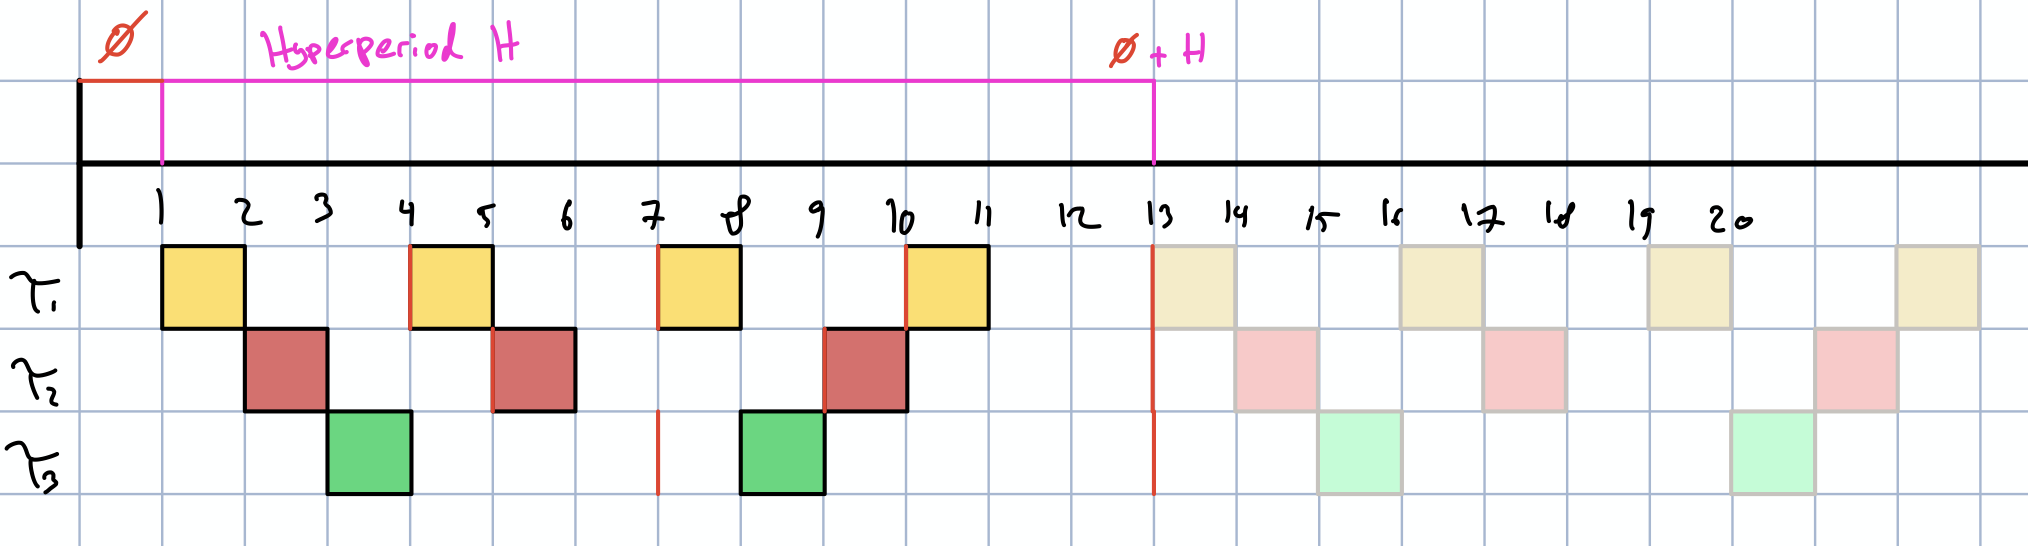
\includegraphics[width=\linewidth]{1-rate-monotonic-schedule}

\item \textbf{Calibrating execution time}

Constraining the execution of the program to use only a single CPU core using taskset was made possible on a macOS system by using a virtual machine. The calibration parameter was set to \textbf{1208} which produced the following output:
\begin{figure}[H]
    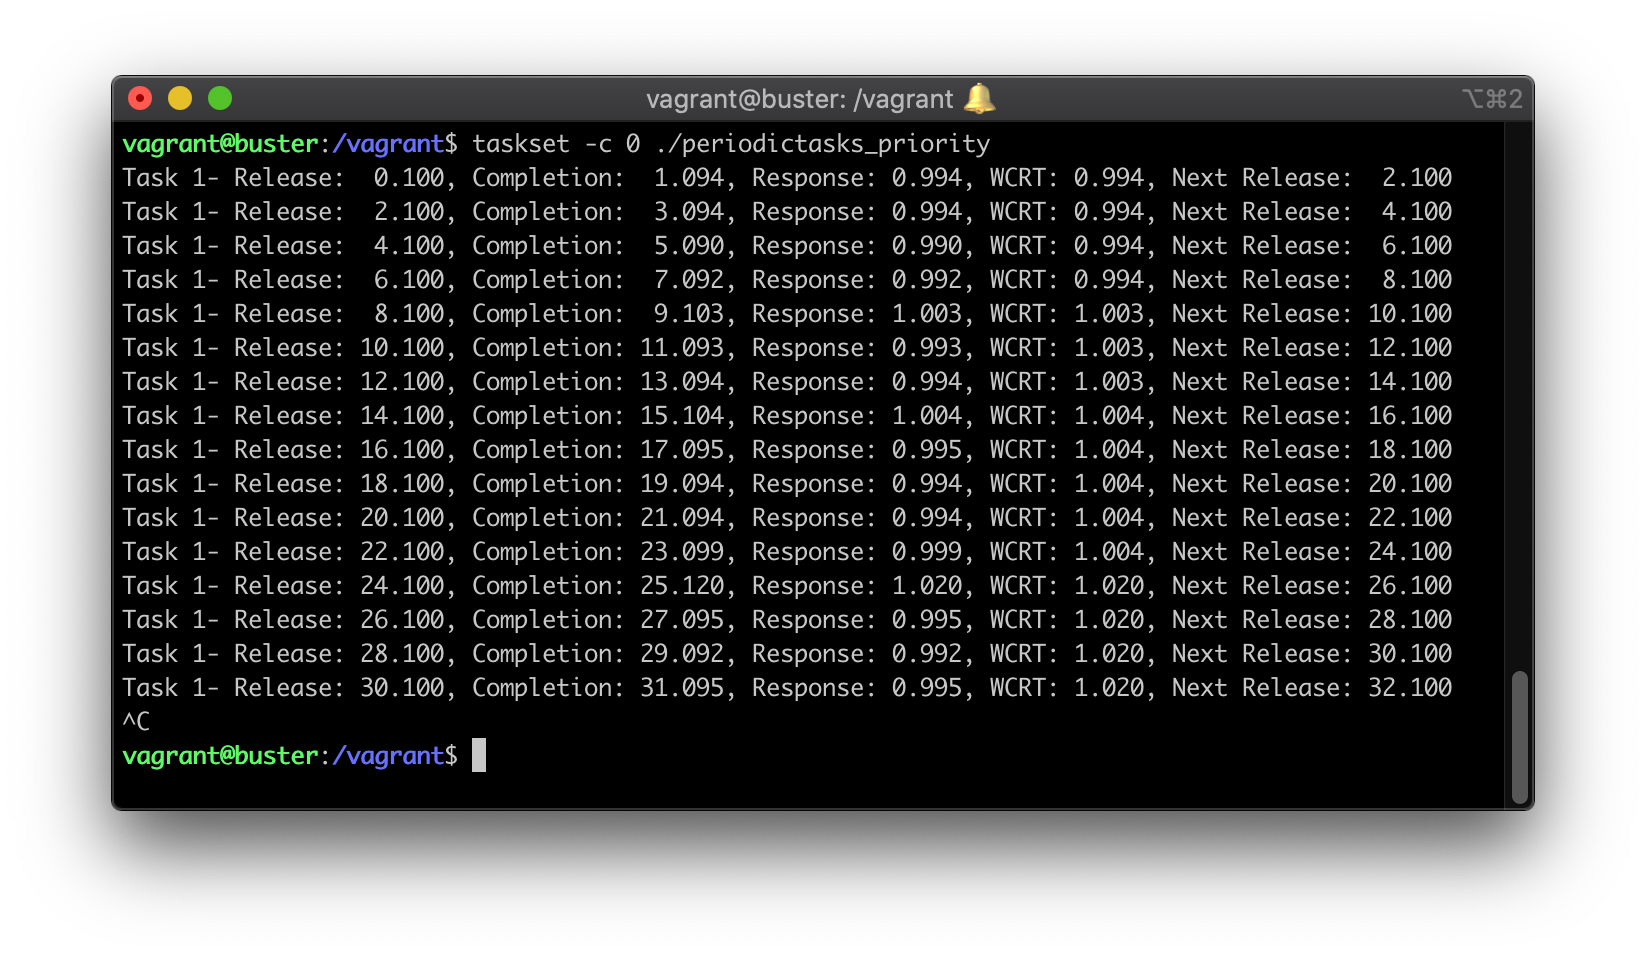
\includegraphics[width=\linewidth]{2-periodictasks-priority-output}
\end{figure}
\item \textbf{Implementing the periodic task set $\Gamma_1$}

Running the rms on a single core produces the following output:
\begin{figure}[H]
    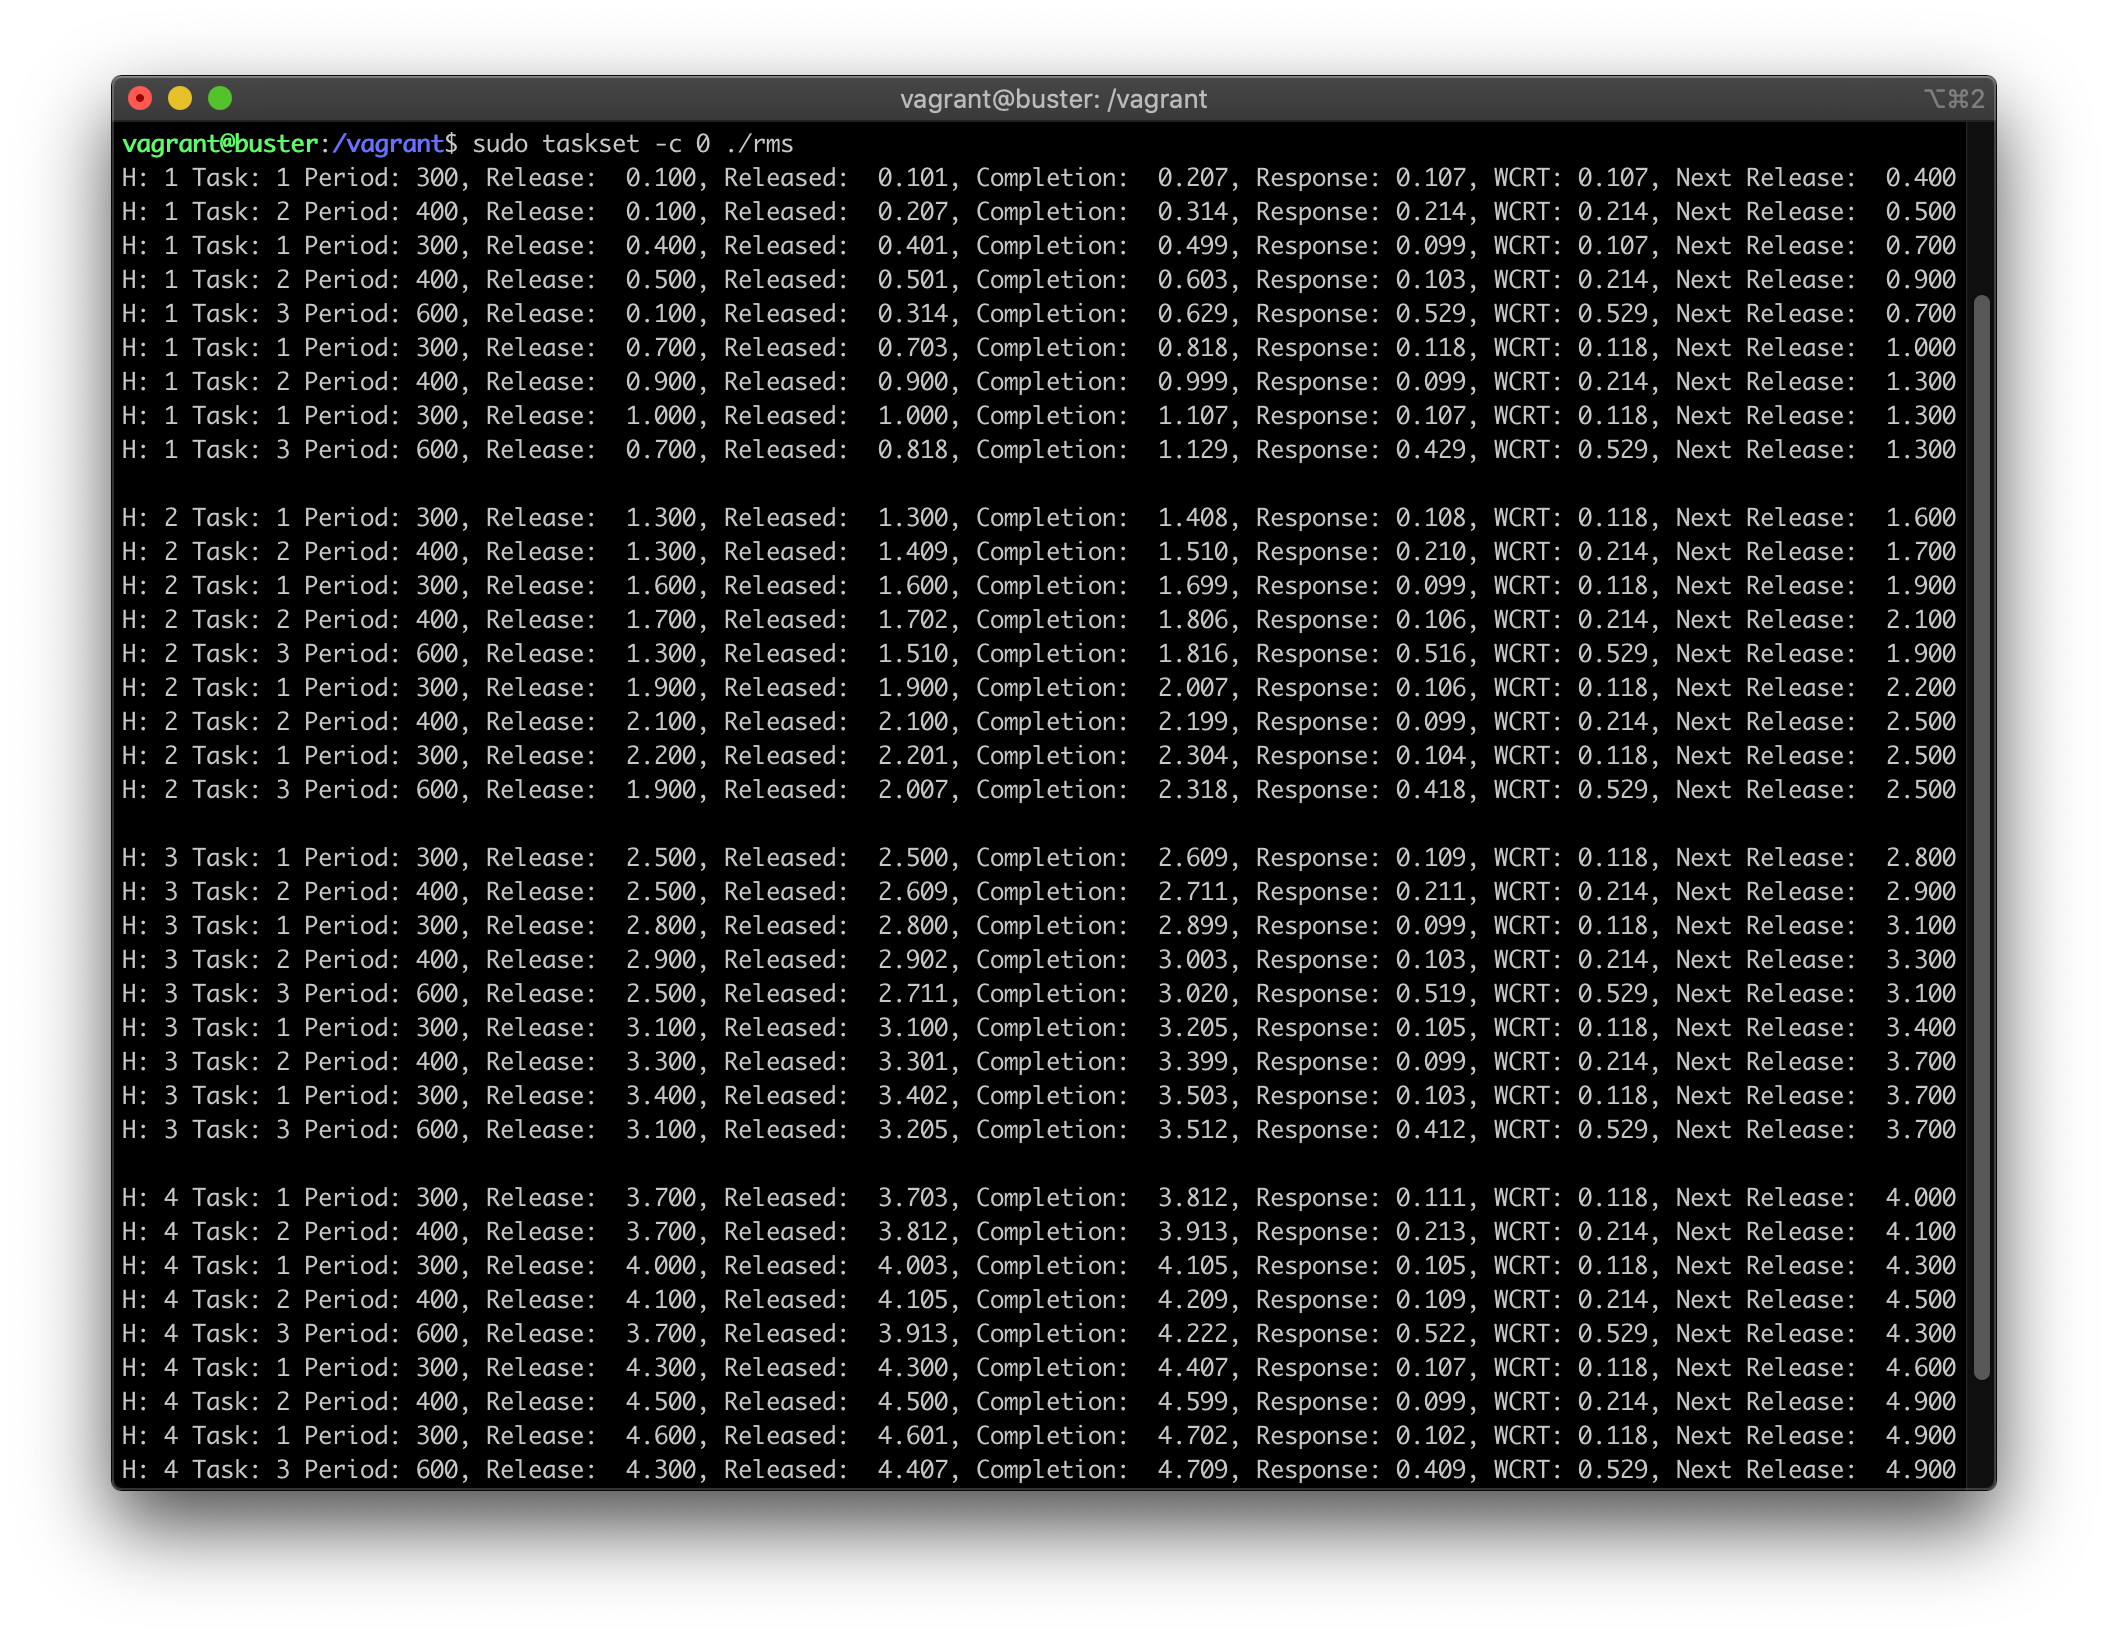
\includegraphics[width=\linewidth]{3-rms-output}
\end{figure}
        Comparing the command output to the theoretical schedule, one can easily verify that indeed the jobs run according to the schematic. While there are minor differences in the order of completion, the \textbf{Released} field reveals when each job was started, which matches the theory.

\item \textbf{Adding the additional task  $\tau_4$}
    A new task $\tau_4$ is added:
        \[\tau_4 = (\phi = 100, T = 1200, C = 200, D = 1200)\]
        Since it has twice the computing time of the other tasks, it can be broken down into two time units and added to the schedule. Starting at $t = 600$ it gets pre-empted by $\tau_1$ due to its higher priority and will have to wait until $t = 1100$ when there are no other tasks pending in order to resume and finish its work.
\begin{figure}[H]
        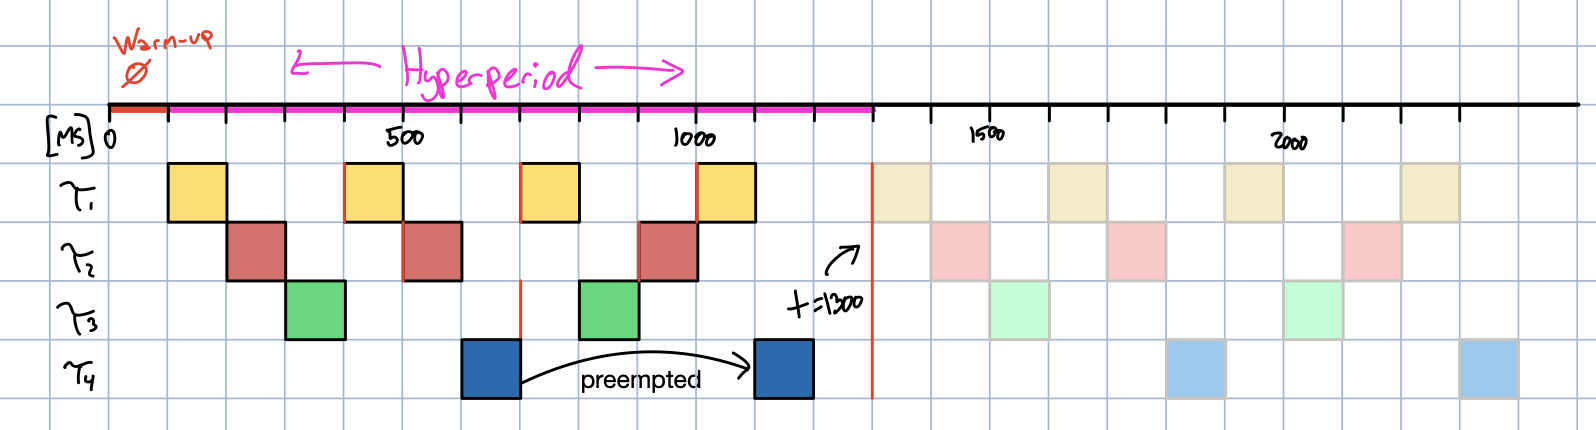
\includegraphics[width=\linewidth]{4-1-rms2-schedule}
\end{figure}
        The output produced by rms2 (the value of Calibration was increased to 1280):
\begin{figure}[H]
        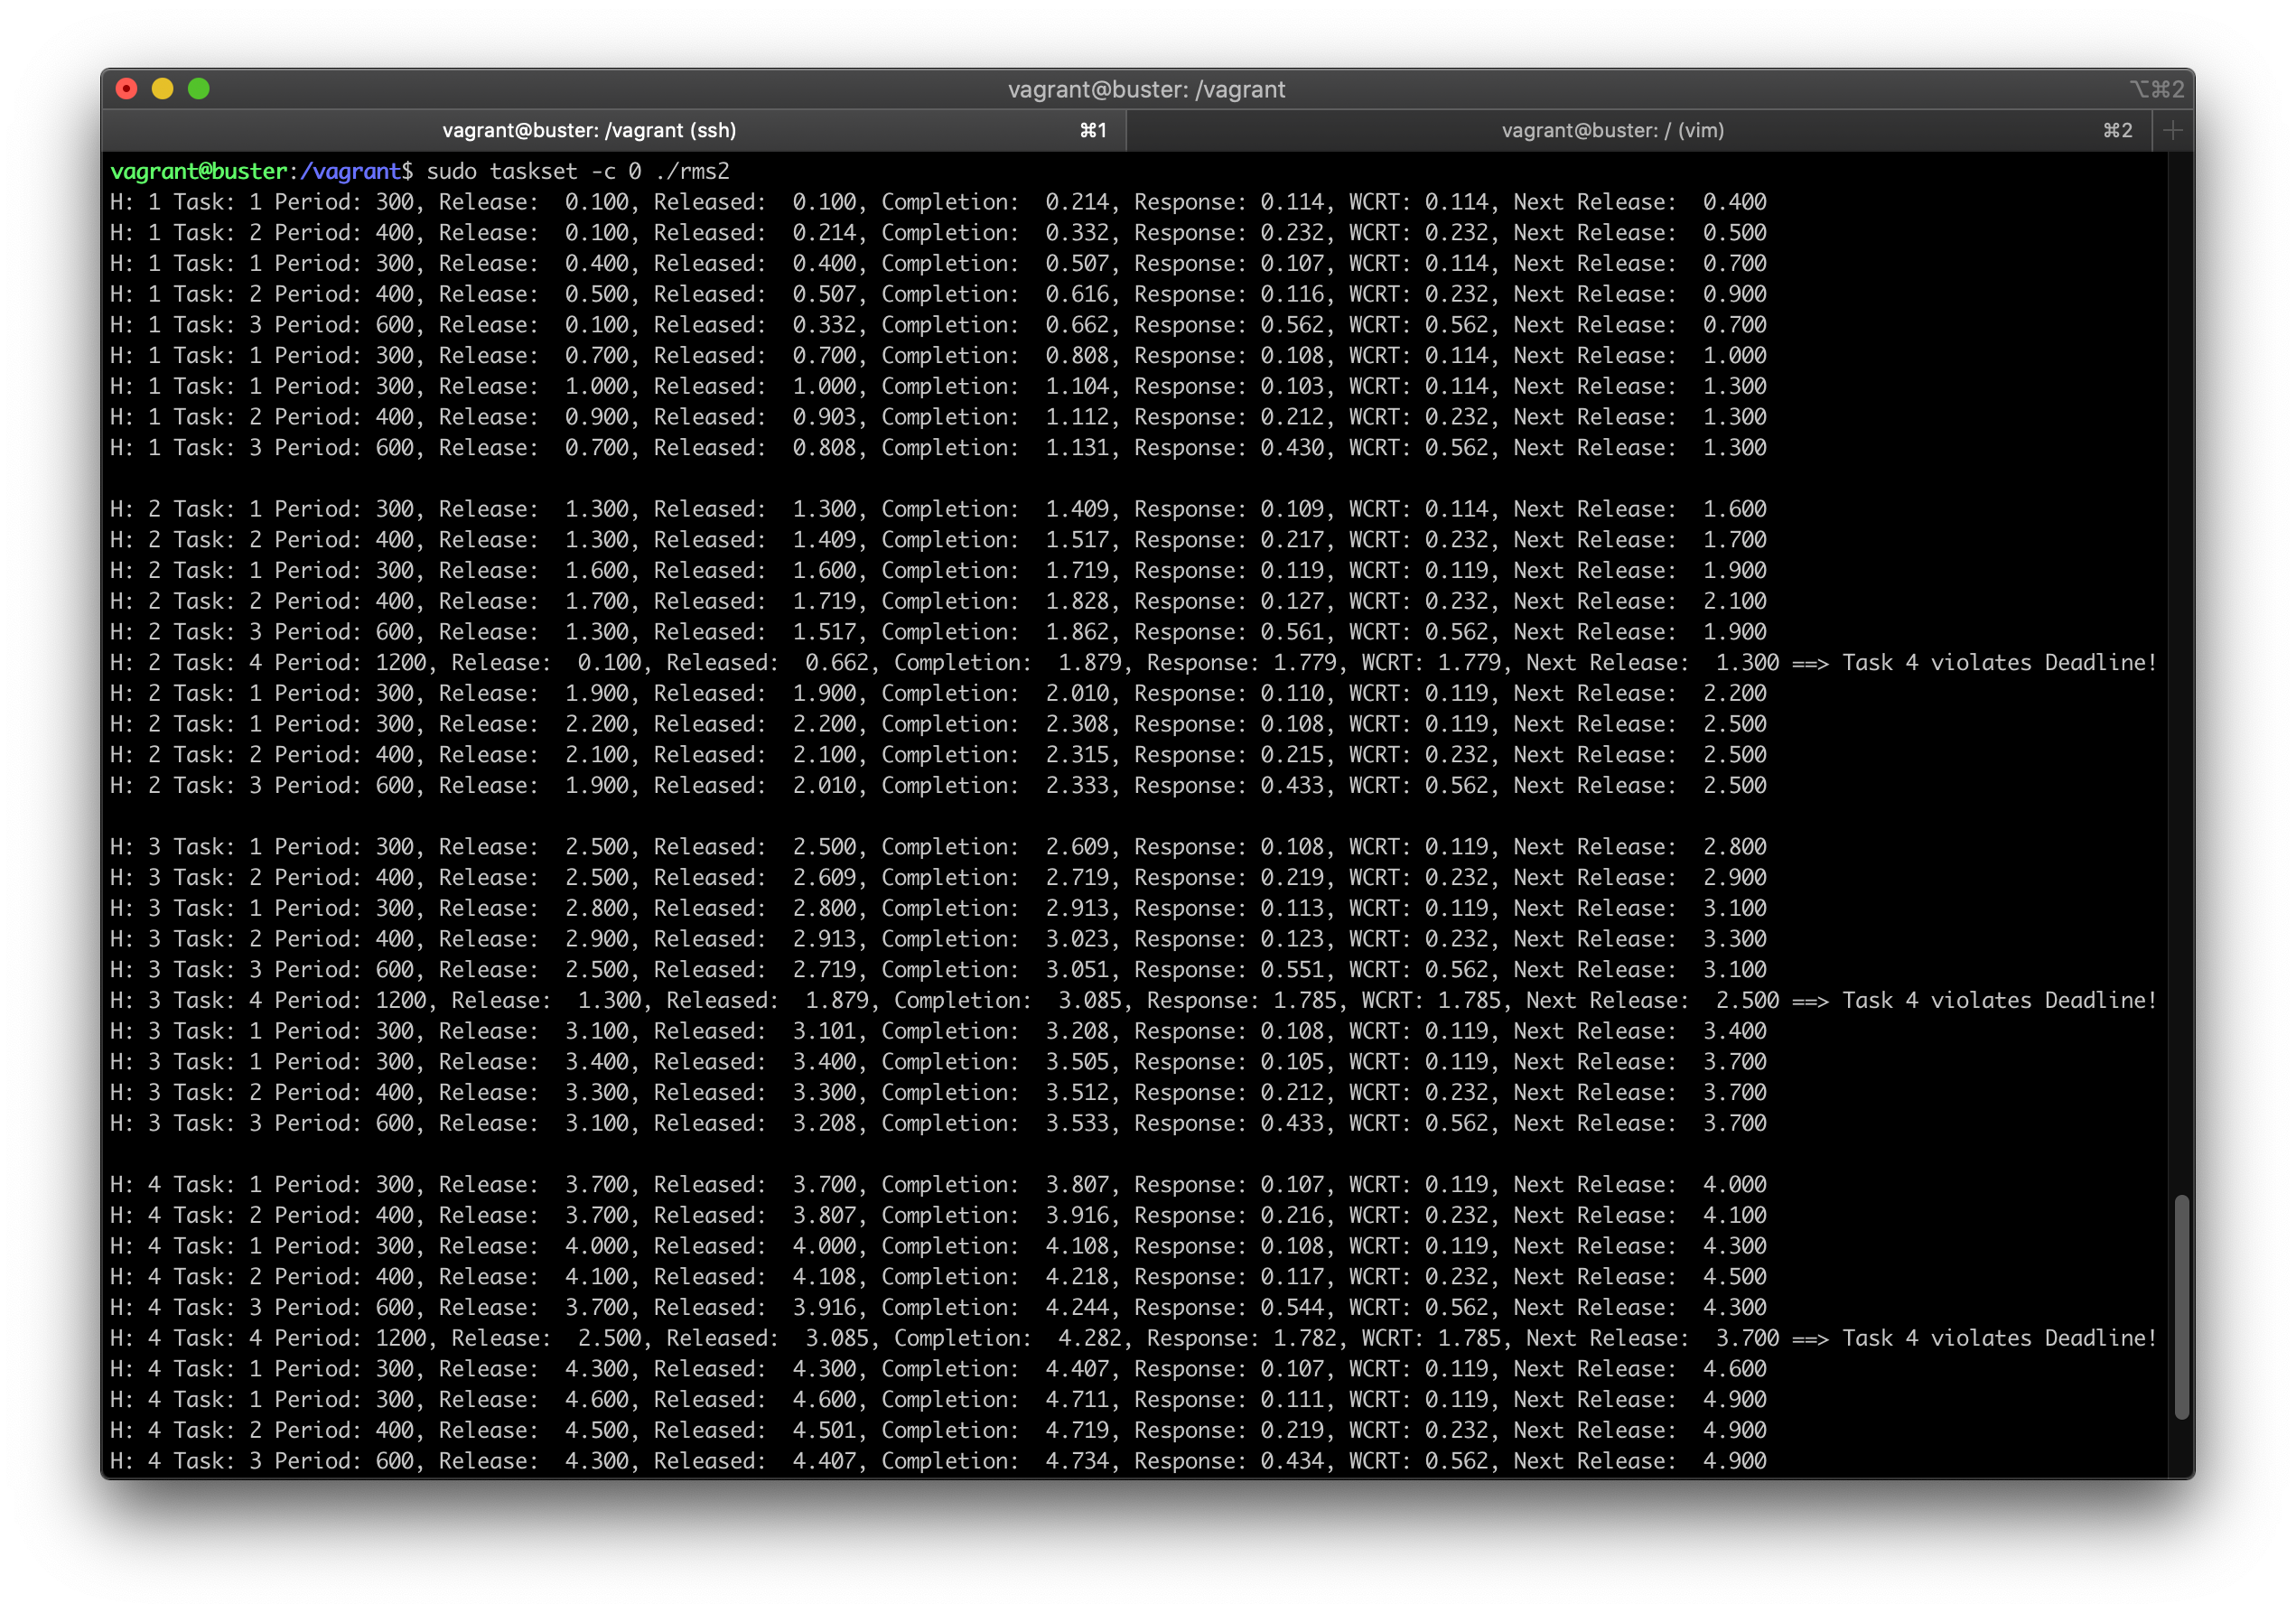
\includegraphics[width=\linewidth]{4-rms2-output}
\end{figure}
        Here one can clearly see the program struggling to keep the deadlines. While $\tau_4$ manages to complete just in time during hyperperiod 1, it doesn't make it in time during hyperperiod 2 and is thus way over deadline when i finally completes at the end of hyperperiod 3. Other tasks also have problems, which is not unexpected since the system is now being utilized at a much higher rate ($U = 11/12 \approx 0.92$).

\end{enumerate}
